\documentclass[12pt, letterpaper]{article}
\usepackage[utf8]{inputenc}
\usepackage{mathtools}          
\usepackage{chngcntr}
\counterwithin*{equation}{section}
\counterwithin*{equation}{subsection}
\usepackage{graphicx}
\graphicspath{{Images/}}
\usepackage{subcaption}
\usepackage{wrapfig}
\usepackage{float}
\usepackage{svg}

\title{ Bo\u{g}azi\c{c}i University\\CMPE 597  \\
   \large  Deep Learning\\
    Final Project Report
}
\author{Alptekin Orbay \\ Student ID: 2017700090}
\date{\today}
\begin{document}


\begin{titlepage}
  \maketitle
\end{titlepage}
\newpage
\tableofcontents
\newpage
\section{Introduction \& Motivation}
	In this study, it is questioned that what is the real meaning of LSTM gates and how the block of LSTM inside affects the hidden states. LSTM gates have their names, but it is not assumed that their functions do not match their names. Also, in \cite{1}, LSTM gates are analyzed with several experiments and it is proposed that Forget and Output gates are the most important ones. However, a recent study \cite{2} also suggest that only forget gate version outperforms basic LSTM type. This results make the situation about gates very confusing. In deep learning view, more gates and more layers makes model stronger if the problem capacity is large enough. The aim of my study is how we must choose true gate structure for different problems type. To illustrate that, I use 6 different type of structure with three datasets which are different level of hardness. 
\section{LSTM Models with Different Gate Structure }
\subsection{Basic LSTM (Basic)}
\begin{align*}
	f &= \sigma(W_f * x_{t} + R_f * h_{t-1} + b_f) \\
	i &= \sigma(W_i * x_{t} + R_i * h_{t-1} + b_i) \\
	z &= \tanh(W_z * x_{t} + R_z * h_{t-1} + b_z) \\ 
	o &= \sigma(W_o * x_{t} + R_o * h_{t-1} + b_o) \\
	c_t &= c_{t-1} * f + z * i \\
	h_t &= tanh(c_t) * o
\end{align*}
\subsection{Only Forget(F)}
\begin{align*}
	f &= \sigma(W_f * x_{t} + R_f * h_{t-1} + b_f) \\
	z &= \tanh(W_z * x_{t} + R_z * h_{t-1} + b_z) \\ 
	c_t &= c_{t-1} * f + z * (1-f) \\
	h_t &= c_t
\end{align*}
\subsection{Forget \& Output(FO)}
\begin{align*}
	f &= \sigma(W_f * x_{t} + R_f * h_{t-1} + b_f) \\
	z &= \tanh(W_z * x_{t} + R_z * h_{t-1} + b_z) \\ 
	o &= \sigma(W_o * x_{t} + R_o * h_{t-1} + b_o) \\
	c_t &= c_{t-1} * f + z * (1-f) \\
	h_t &= tanh(c_t) * o
\end{align*}
\subsection{Input \& Output(IO)}
\begin{align*}
	i &= \sigma(W_i * x_{t} + R_i * h_{t-1} + b_i) \\
	z &= \tanh(W_z * x_{t} + R_z * h_{t-1} + b_z) \\ 
	o &= \sigma(W_o * x_{t} + R_o * h_{t-1} + b_o) \\
	c_t &= c_{t-1}*- * z  \\
	h_t &= tanh(c_t) * o
\end{align*}
\subsection{Only Output(O)}
\begin{align*}
	z &= \tanh(W_z * x_{t} + R_z * h_{t-1} + b_z) \\ 
	o &= \sigma(W_o * x_{t} + R_o * h_{t-1} + b_o) \\
	c_t &= c_{t-1} + z  \\
	h_t &= tanh(c_t) * o
\end{align*}
\subsection{Forget \& Output with different order(myFO)}
\begin{align*}
	f &= \sigma(W_f * x_{t} + R_f * h_{t-1} + b_f) \\
	z &= \tanh(W_z * x_{t} + R_z * h_{t-1} + b_z) \\ 
	o &= \sigma(W_o * x_{t} + R_o * h_{t-1} + b_o) \\
	c_t &= f * (c_{t-1} + z)  \\
	h_t &= tanh(c_t) * o
\end{align*}
\section{Experiments}
	For creating different type of LSTM types, cite{4} is the source of inspiration. I modified basic LSTM and construct other models. I did some tricks to visualize the gates.
\subsection{Parity Check}
\subsubsection{Dataset}
	This dataset is an artificial dataset. This problem needs to curriculum learning to solve. Also, it should be solved with only one hidden state. However, it would be challenging as LSTM can learn statistically so it must give hard response like electrical gates. But, this example is good for illustration of functions of gates and hidden states. As the number of hidden unit number increases, the interpolation of gates become harder. 
\subsubsection{Setup}
	The training set and test set sampled from binomial distribution with different lengths. All the models start training with length 2 and finished with length 8. As they learn current length, the next length sized inputs are fed to model. The test is done with 100-length sequences to see which model make generalization better. Actually, all models would learn the training samples very well, and they all are expected to perform very well with 9 or 10 length sequences. The point is that which gates addition and deletion makes the model more generic. We know that LSTM gates can give soft decisions very well, whether hard decisions are also enabled. In addition to that, it could help to learn which gates makes more affect on hidden states and  why.
\subsubsection{Results}

\begin{center}
\begin{tabular}{ |c|c|c|c|c|c|c|  } 
 \hline
3-HiddenUnit & Basic  &  F     &  FO     & myFO  & IO    &    O  \\ \hline
Accuracy & 96.7   &  91.8  &  99.89  & 98.22  & 80.7  & 74.47 \\ \hline
Iteration Number & 267    &  5942  &   55    & 4118  	& 6718  & 47.419 \\
 \hline
\end{tabular}
\end{center}

\begin{center}
\begin{tabular}{ |c|c|c|c|c|c|c|  } 
 \hline
1-HiddenUnit      & Basic  &  F     &  FO       & myFO  & IO    &    O  \\ \hline 
Accuracy          & 81.7    &  99.85   &  100      & 99.93  & -  & - \\ \hline
Iteration Number  & 76     &  67    &   91      & 555   & 
-  & -\\
 \hline
\end{tabular}
\end{center}

	The results show that LSTM is very suitable for over-fitting. If the model uses more hidden units than needed which is very hard to determine for every problem, it directly loses its generalization. With 3 hidden unit, FO and invFO is the best ones as forget gate and output gate are the most important ones. Input gate is not required to solve this problem as seen in results. Basic LSTM is not best although it seems to be the most powerful. While 3 hidden unit pushes the model lazy learning and input gate is also harmful. Another deduction is that forget gate is need to solve this type of problems. With one hidden layer, forget gate makes all the job itself.

\begin{figure}[h]
    \centering
    \begin{subfigure}[b]{0.3\textwidth}
        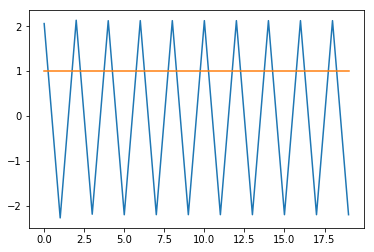
\includegraphics[width=\textwidth]{f1}
        \label{fig:gull}
    \end{subfigure}
    ~ %add desired spacing between images, e. g. ~, \quad, \qquad, \hfill etc. 
      %(or a blank line to force the subfigure onto a new line)
    \begin{subfigure}[b]{0.3\textwidth}
        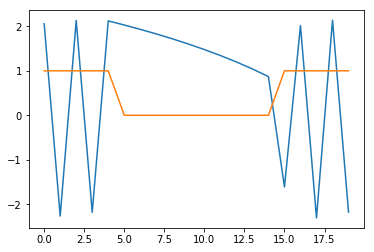
\includegraphics[width=\textwidth]{f2}
        \label{fig:tiger}
    \end{subfigure}
    ~ %add desired spacing between images, e. g. ~, \quad, \qquad, \hfill etc. 
    %(or a blank line to force the subfigure onto a new line)
    \begin{subfigure}[b]{0.3\textwidth}
        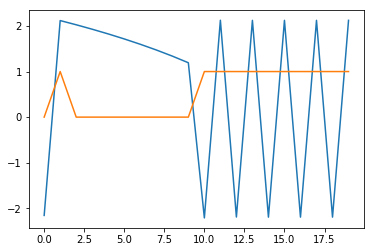
\includegraphics[width=\textwidth]{f3}
        \label{fig:mouse}
    \end{subfigure}
    \caption{Only-F.Blues is hidden states whereas orange is input.}\label{fig:animals}
\end{figure}

\begin{figure}[h]
    \centering
    \begin{subfigure}[b]{0.3\textwidth}
        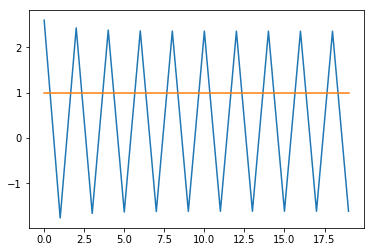
\includegraphics[width=\textwidth]{basic1}
        \label{fig:gull}
    \end{subfigure}
    ~ %add desired spacing between images, e. g. ~, \quad, \qquad, \hfill etc. 
      %(or a blank line to force the subfigure onto a new line)
    \begin{subfigure}[b]{0.3\textwidth}
        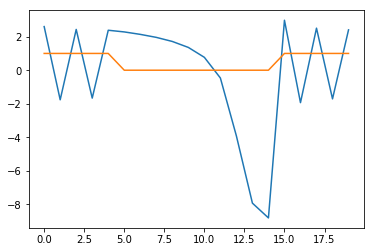
\includegraphics[width=\textwidth]{basic2}
        \label{fig:tiger}
    \end{subfigure}
    ~ %add desired spacing between images, e. g. ~, \quad, \qquad, \hfill etc. 
    %(or a blank line to force the subfigure onto a new line)
    \begin{subfigure}[b]{0.3\textwidth}
        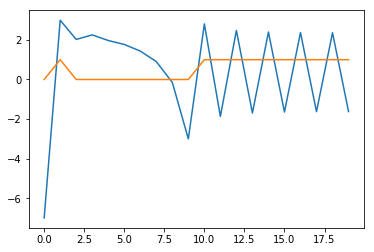
\includegraphics[width=\textwidth]{basic3}
        \label{fig:mouse}
    \end{subfigure}
    \caption{Basic-LSTM.Blues is hidden states whereas orange is input.}\label{fig:animals}
\end{figure}

\begin{figure}[h]
    \centering
    \begin{subfigure}[b]{0.3\textwidth}
        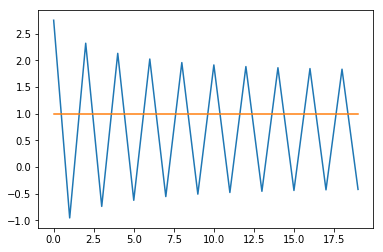
\includegraphics[width=\textwidth]{fo1}
        \label{fig:gull}
    \end{subfigure}
    ~ %add desired spacing between images, e. g. ~, \quad, \qquad, \hfill etc. 
      %(or a blank line to force the subfigure onto a new line)
    \begin{subfigure}[b]{0.3\textwidth}
        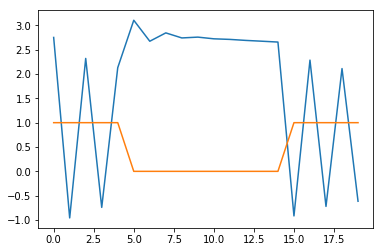
\includegraphics[width=\textwidth]{fo2}
        \label{fig:tiger}
    \end{subfigure}
    ~ %add desired spacing between images, e. g. ~, \quad, \qquad, \hfill etc. 
    %(or a blank line to force the subfigure onto a new line)
    \begin{subfigure}[b]{0.3\textwidth}
        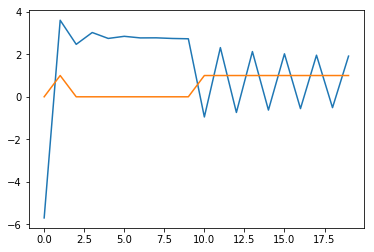
\includegraphics[width=\textwidth]{fo3}
        \label{fig:mouse}
    \end{subfigure}
    \caption{Output-Forget LSTM.Blues is hidden states whereas orange is input.}\label{fig:animals}
\end{figure}

\begin{figure}[h]
    \centering
    \begin{subfigure}[b]{0.3\textwidth}
        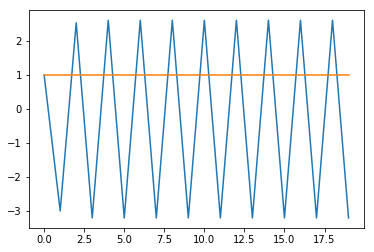
\includegraphics[width=\textwidth]{of1}
        \label{fig:gull}
    \end{subfigure}
    ~ %add desired spacing between images, e. g. ~, \quad, \qquad, \hfill etc. 
      %(or a blank line to force the subfigure onto a new line)
    \begin{subfigure}[b]{0.3\textwidth}
        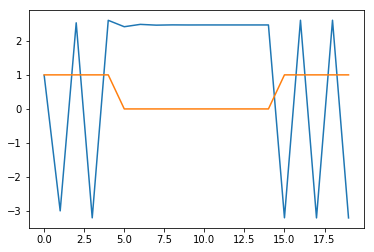
\includegraphics[width=\textwidth]{of2}
        \label{fig:tiger}
    \end{subfigure}
    ~ %add desired spacing between images, e. g. ~, \quad, \qquad, \hfill etc. 
    %(or a blank line to force the subfigure onto a new line)
    \begin{subfigure}[b]{0.3\textwidth}
        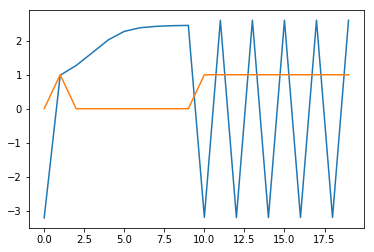
\includegraphics[width=\textwidth]{of3}
        \label{fig:mouse}
    \end{subfigure}
    \caption{myFO.Blues is hidden states whereas orange is input.}
  \label{fig:animals}
\end{figure}

This graphs are indication of hidden states through time. The results are suggested that output-forget gate combination performs without leak. Basic-LSTM and Only-forget gate have leaks that results in failure after some repeated zeros. It is seen clearly, for problems, the model must be chosen very carefully for stable learning. Note that the order of the gates are important as the learning time are very different. Also, the output-forget gate oscillations get smaller. It could be problem for long sequences.

\subsubsection{Gate Results}
\begin{figure}[h]
    \centering
    \begin{subfigure}[b]{0.3\textwidth}
        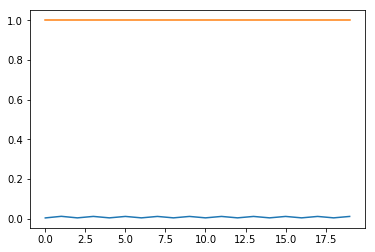
\includegraphics[width=\textwidth]{basic_f1}
        \label{fig:gull}
    \end{subfigure}
    ~ %add desired spacing between images, e. g. ~, \quad, \qquad, \hfill etc. 
      %(or a blank line to force the subfigure onto a new line)
    \begin{subfigure}[b]{0.3\textwidth}
        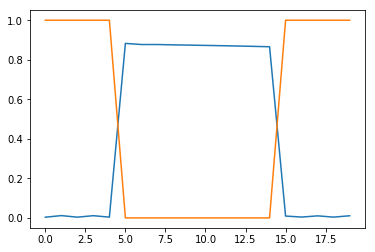
\includegraphics[width=\textwidth]{basic_f2}
        \label{fig:tiger}
    \end{subfigure}
    ~ %add desired spacing between images, e. g. ~, \quad, \qquad, \hfill etc. 
    %(or a blank line to force the subfigure onto a new line)
    \begin{subfigure}[b]{0.3\textwidth}
        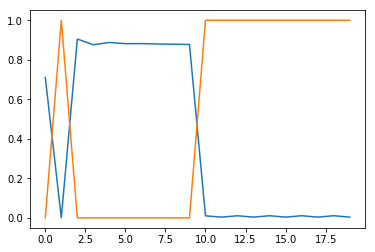
\includegraphics[width=\textwidth]{basic_f3}
        \label{fig:mouse}
    \end{subfigure}
    \caption{Basic LSTM forget gate. Blue one is hidden state and orange one is input.}\label{fig:animals}
\end{figure}
\begin{figure}[h]
    \centering
    \begin{subfigure}[b]{0.3\textwidth}
        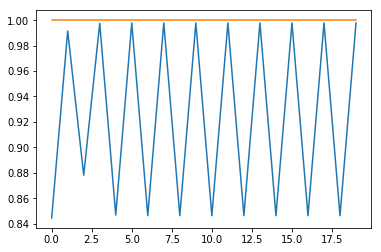
\includegraphics[width=\textwidth]{of_f1}
        \label{fig:gull}
    \end{subfigure}
    ~ %add desired spacing between images, e. g. ~, \quad, \qquad, \hfill etc. 
      %(or a blank line to force the subfigure onto a new line)
    \begin{subfigure}[b]{0.3\textwidth}
        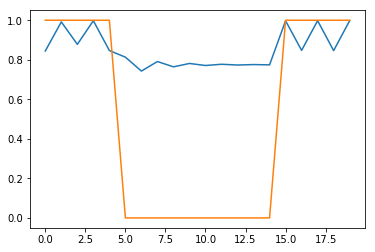
\includegraphics[width=\textwidth]{of_f2}
        \label{fig:tiger}
    \end{subfigure}
    ~ %add desired spacing between images, e. g. ~, \quad, \qquad, \hfill etc. 
    %(or a blank line to force the subfigure onto a new line)
    \begin{subfigure}[b]{0.3\textwidth}
        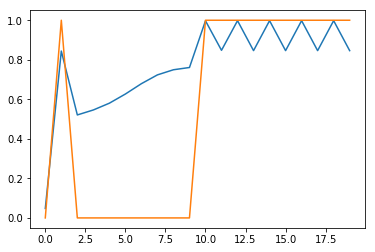
\includegraphics[width=\textwidth]{of_f3}
        \label{fig:mouse}
    \end{subfigure}
    \caption{myFO.Blues is forget gates whereas orange is input.}\label{fig:animals}
\end{figure}
\begin{figure}[h]
    \centering
    \begin{subfigure}[b]{0.3\textwidth}
        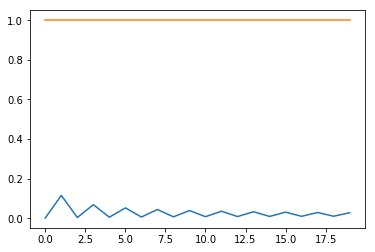
\includegraphics[width=\textwidth]{fo_f1}
        \label{fig:gull}
    \end{subfigure}
    ~ %add desired spacing between images, e. g. ~, \quad, \qquad, \hfill etc. 
      %(or a blank line to force the subfigure onto a new line)
    \begin{subfigure}[b]{0.3\textwidth}
        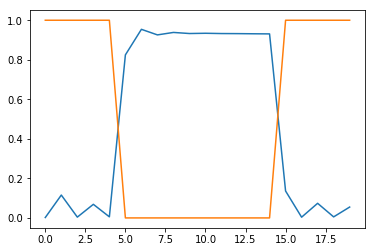
\includegraphics[width=\textwidth]{fo_f2}
        \label{fig:tiger}
    \end{subfigure}
    ~ %add desired spacing between images, e. g. ~, \quad, \qquad, \hfill etc. 
    %(or a blank line to force the subfigure onto a new line)
    \begin{subfigure}[b]{0.3\textwidth}
        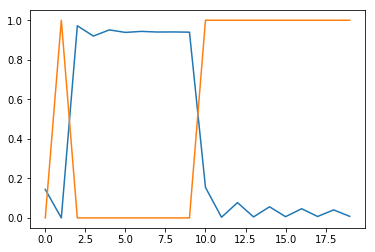
\includegraphics[width=\textwidth]{fo_f3}
        \label{fig:mouse}
    \end{subfigure}
    \caption{FO.Blues is forget gates whereas orange is input.}\label{fig:animals}
\end{figure}
\begin{figure}[h]
    \centering
    \begin{subfigure}[b]{0.3\textwidth}
        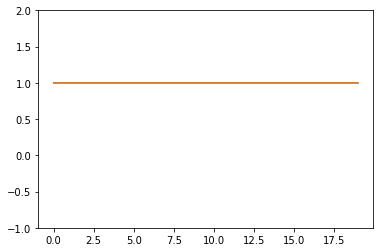
\includegraphics[width=\textwidth]{of_c1}
        \label{fig:gull}
    \end{subfigure}
    ~ %add desired spacing between images, e. g. ~, \quad, \qquad, \hfill etc. 
      %(or a blank line to force the subfigure onto a new line)
    \begin{subfigure}[b]{0.3\textwidth}
        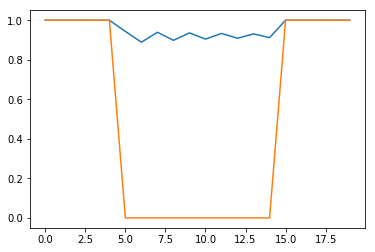
\includegraphics[width=\textwidth]{of_c2}
        \label{fig:tiger}
    \end{subfigure}
    ~ %add desired spacing between images, e. g. ~, \quad, \qquad, \hfill etc. 
    %(or a blank line to force the subfigure onto a new line)
    \begin{subfigure}[b]{0.3\textwidth}
        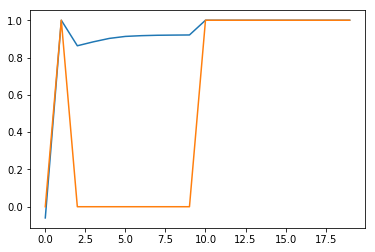
\includegraphics[width=\textwidth]{of_c3}
        \label{fig:mouse}
    \end{subfigure}
    \caption{myFO.Blues is candidate state whereas orange is input.}\label{fig:animals}
\end{figure}


\begin{figure}[H]
    \centering
    \begin{subfigure}[b]{0.3\textwidth}
        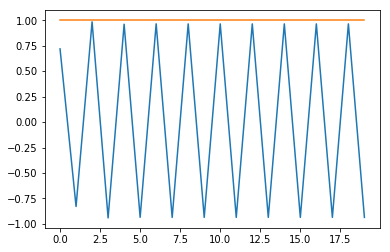
\includegraphics[width=\textwidth]{fo_c1}
        \label{fig:gull}
    \end{subfigure}
    ~ %add desired spacing between images, e. g. ~, \quad, \qquad, \hfill etc. 
      %(or a blank line to force the subfigure onto a new line)
    \begin{subfigure}[b]{0.3\textwidth}
        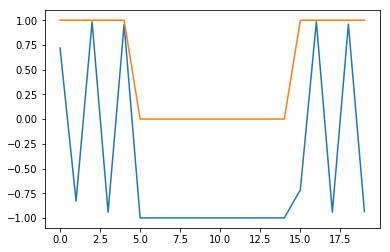
\includegraphics[width=\textwidth]{fo_c2}
        \label{fig:tiger}
    \end{subfigure}
    ~ %add desired spacing between images, e. g. ~, \quad, \qquad, \hfill etc. 
    %(or a blank line to force the subfigure onto a new line)
    \begin{subfigure}[b]{0.3\textwidth}
        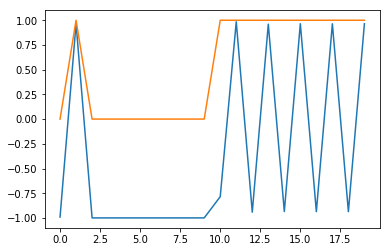
\includegraphics[width=\textwidth]{fo_c3}
        \label{fig:mouse}
    \end{subfigure}
    \caption{FO.Blues is candidate states whereas orange is input.}\label{fig:animals}
\end{figure}



	In this section, gates results are investigated to understand why forget-output combination outperforms basic LSTM and how LSTM responds to change of order. In results, it is seen that order makes the importance also. In graphs of candidate state and forget gates, one of them is performing in hard manner which we want to solve this problem. One of the gates are always in saturation mode. In myFO, forget gate is saturating and dominant. In normal FO, candidate state is always saturating and dominating. In some extreme cases, the areas those are not saturated lead to minor mistake that explains why all the accuracy results for forget and output combination are not 100.
	
\newpage
\subsection{MNIST Classification}
\subsubsection{Dataset}
	This dataset is the one of the most known benchmark datasets. The images are 8 by 8 and LSTM is fed with input size 8 and sequence size 8.
\subsubsection{Setup}
	As LSTM converges fast, I give the best results of each method after 10 experiments for each. I used early stopping for regularization and Adam optimizer is used with learning rate 0.001.
I used different hidden units. For 30, the results are very close to state of the art. So, it is determined as upper limit. For 1, there is also learning so it is chosen for bottom limit. For 15, it may be seen that which model is robust limited source.
\subsubsection{Results}
\begin{center}
\begin{tabular}{ |c|c|c|c|c|c|c|  } 
 \hline
Unit - Accuracy   & Basic  &  F     &  FO     & myFO  & IO    &    O  \\ \hline 
30        & 97.22   &  96.22  &  96.71  & 96.96  & 96.96  & 95.7 \\ \hline
15       &    93.93 &   92.67 &    90.2   & 95.2   	& 95.45  &   93.68  \\ \hline
1  	 &     69.94    &    20.95     &     21.21   &  26.51        & 24.49      & 18.68\\
 \hline
\end{tabular}
\end{center}
	First of all, Basic LSTM is the best model for MNIST as this dataset is more realistic, but toy. All the models can overcome this challenge. But, when hidden size is sufficient and dataset is more suitable for relax learning, gates importance diminishes. Interestingly, IO can perform as good as models with forget gates. When the model capacity is decreased with hidden size dramatically, Basic LSTM can give meaningful results as it contains more parameters. It can be said that Basic LSTM can be applied safely for
problem in which the prior knowledge is missing. In some cases, other models can performs well, but, in average,Basic LSTM may give the best results. 
\subsection{Sentiment Analysis}
\subsubsection{Dataset}
	This dataset is the most realistic and most big one in my experiments. Word embedding is also used and the dataset is fetched from \cite{3} with embeddings. It contains IMDB movie reviews and there are 25000 reviews. The number of positive and negative reviews are the same. 23000 reviews are train-set and 2000 reviews are left as test set. Also, Glove word-embedding is used whose embedding size is 50. And the sequence length are variable and maximum is 250.
\subsubsection{Setup}
I also deal with this dataset for another course to learn regularization in RNNs. My best accuracy with this dataset with Basic LSTM, variational dropout \cite{4} and a set optimizer is about 85. From this experience, I fix the hidden layer size 64 and
Adam as optimizer. As the experiments takes too much time, the fine-tunning is not done optimally. Models are trained sufficiently for each and until converges, the experiments repeated.
\subsubsection{Results}
\begin{center}
\begin{tabular}{ |c|c|c|c|c|c|c|  } 
 \hline
Unit - Accuracy   & Basic  &  F     &  FO     & myFO  & IO    &    O  \\ \hline 
30        & 83.61   &  85.32  &  83.05  & 80.25  & 83.13  & 63.28 \\ \hline
 \hline
\end{tabular}
\end{center}
	Interestingly, I used several method to increase accuracy for Basic LSTM. However, only-F gives the better results without any fine tunning. Also, only output-gate type is the weakest one.
\section{Conclusion}
	To sum up, my experiments are consistent with the results in \cite{1} and \cite{2}. The most important gates are forget and output in my results in classical configuration. It is important to verify my experiments. Also, only forget gate performs as good as basic LSTM. However, my detailed analysis shows that gate order and dataset together determines the important ones. Also, for some problems, only disabling some gates give higher results. It is important that applying regularization methods reduces the speed and
performance. So, first disabling some gates save time. Also, to find the best model for dataset, it is more appropriate to start with basic LSTM and removing some gate. Starting with only forget gate and adding additional gates can results in non-optimal hyper-parameter. To measure the hardness of problem, Basic one should be preferred. Also, theoretically, LSTM gates can bu used in saturation mode. It enables understanding gates and LSTM models can easily implemented with electronic gates.  
\section{References}


\begin{thebibliography}{9}
\bibitem{1} 
Klaus Greff, Rupesh Kumar Srivastava, Jan Koutník, Bas R. Steunebrink, Jürgen Schmidhuber(2015).LSTM: A Search Space Odyssey
\textit{ arXiv:1503.04069 }


\bibitem{2} 
Jos van der Westhuizen, Joan Lasenby.(2018)  The unreasonable effectiveness of the forget gate. \textit{ 	arXiv:1804.04849}

 
\bibitem{3} 
https://github.com/adeshpande3/LSTM-Sentiment-Analysis

\bibitem{4}
https://github.com/KnHuq/Dynamic-Tensorflow-Tutorial

\bibitem{5} 
Yarin Gal, Zoubin Ghahramani(2017).A Theoretically Grounded Application of Dropout in Recurrent Neural Networks 
\textit{arXiv:1512.05287 }. 
\end{thebibliography}

\section{Code}

\subsection{Basic LSTM}
\begin{verbatim}
class LSTM_cell(object):

    """
    LSTM cell object which takes 3 arguments for initialization.
    input_size = Input Vector size
    hidden_layer_size = Hidden layer size
    target_size = Output vector size

    """

    def __init__(self, input_size, hidden_layer_size, target_size):

        # Initialization of given values
        self.input_size = input_size
        self.hidden_layer_size = hidden_layer_size
        self.target_size = target_size


        self.Wf = tf.Variable(tf.zeros(
            [self.input_size, self.hidden_layer_size]))
        self.Uf = tf.Variable(tf.zeros(
            [self.hidden_layer_size, self.hidden_layer_size]))
        self.bf = tf.Variable(tf.zeros([self.hidden_layer_size]))        

        
        self.Wi = tf.Variable(tf.zeros(
            [self.input_size, self.hidden_layer_size]))
        self.Ui = tf.Variable(tf.zeros(
            [self.hidden_layer_size, self.hidden_layer_size]))
        self.bi = tf.Variable(tf.zeros([self.hidden_layer_size]))        

        
        self.Wc = tf.Variable(tf.zeros(
            [self.input_size, self.hidden_layer_size]))
        self.Uc = tf.Variable(tf.zeros(
            [self.hidden_layer_size, self.hidden_layer_size]))
        self.bc = tf.Variable(tf.zeros([self.hidden_layer_size]))
        
        self.Wog = tf.Variable(tf.zeros(
            [self.input_size, self.hidden_layer_size]))
        self.Uog = tf.Variable(tf.zeros(
            [self.hidden_layer_size, self.hidden_layer_size]))
        self.bog = tf.Variable(tf.zeros([self.hidden_layer_size]))
        
          # Weights for output layers
        self.Wo = tf.Variable(tf.truncated_normal([self.hidden_layer_size, self.target_size], mean=0, stddev=.01))
        self.bo = tf.Variable(tf.truncated_normal([self.target_size], mean=0, stddev=.01))
        
        
        self._inputs = tf.placeholder(tf.float32,
                                      shape=[None, None, self.input_size],
                                      name='inputs')

        # Processing inputs to work with scan function
        self.processed_input = process_batch_input_for_RNN(self._inputs)

        '''
        Initial hidden state's shape is [1,self.hidden_layer_size]
        In First time stamp, we are doing dot product with weights to
        get the shape of [batch_size, self.hidden_layer_size].
        For this dot product tensorflow use broadcasting. But during
        Back propagation a low level error occurs.
        So to solve the problem it was needed to initialize initial
        hiddden state of size [batch_size, self.hidden_layer_size].
        So here is a little hack !!!! Getting the same shaped
        initial hidden state of zeros.
        '''

        self.initial_hidden = self._inputs[:, 0, :]
        self.initial_hidden= tf.matmul(
            self.initial_hidden, tf.zeros([input_size, hidden_layer_size]))
        
        
        self.initial_hidden=tf.stack([self.initial_hidden,self.initial_hidden,self.initial_hidden])
    # Function for LSTM cell.
    def Lstm(self, previous_hidden_memory_tuple, x):
        """
        This function takes previous hidden state and memory tuple with input and
        outputs current hidden state.
        """
        
        previous_hidden_state,c_prev,_=tf.unstack(previous_hidden_memory_tuple)

        #Forget Gate
        f =  tf.sigmoid(
            tf.matmul(x,self.Wf)+tf.matmul(previous_hidden_state,self.Uf) + self.bf)
        
        i =  tf.sigmoid(
            tf.matmul(x,self.Wi)+tf.matmul(previous_hidden_state,self.Ui) + self.bi)
          
        c_ = tf.tanh(
            tf.matmul(x,self.Wc)+tf.matmul(previous_hidden_state,self.Uc) + self.bc)
       
        o = tf.sigmoid(tf.matmul(x,self.Wog)+tf.matmul(previous_hidden_state,self.Uog) + self.bog)
            
        #Current Hidden state
        c = f *c_prev +  c_* i
        current_hidden_state = tf.tanh(c) * o


        return tf.stack([current_hidden_state,c,f])

    # Function for getting all hidden state.
    def get_states(self):
        """
        Iterates through time/ sequence to get all hidden state
        """

        # Getting all hidden state throuh time
        all_hidden_states = tf.scan(self.Lstm,
                                    self.processed_input,
                                    initializer=self.initial_hidden,
                                    name='states')
        all_hidden_state=all_hidden_states[:,0,:,:]
        
        return all_hidden_state,all_hidden_states[:,2,:,:]

    # Function to get output from a hidden layer
    def get_output(self, hidden_state):
        """
        This function takes hidden state and returns output
        """
        output = tf.matmul(hidden_state, self.Wo) + self.bo

        return output

    # Function for getting all output layers
    def get_outputs(self):
        """
        Iterating through hidden states to get outputs for all timestamp
        """
        all_hidden_states,gates = self.get_states()

        all_outputs = tf.map_fn(self.get_output, all_hidden_states)

        return all_outputs,gates


# Function to convert batch input data to use scan ops of tensorflow.
def process_batch_input_for_RNN(batch_input):
    """
    Process tensor of size [5,3,2] to [3,5,2]
    """
    batch_input_ = tf.transpose(batch_input, perm=[2, 0, 1])
    X = tf.transpose(batch_input_)

    return X
\end{verbatim}

\subsection{Modification on Basic LSTM}

\subsubsection{F}
\begin{verbatim}
    def Lstm(self, previous_hidden_memory_tuple, x):
        """
        This function takes previous hidden state and memory tuple with input and
        outputs current hidden state.
        """
        
        previous_hidden_state,c_prev,_=tf.unstack(previous_hidden_memory_tuple)

        #Forget Gate
        f= tf.sigmoid(
            tf.matmul(x,self.Wf)+tf.matmul(previous_hidden_state,self.Uf) + self.bf 
        )
        

        c_ = tf.tanh(
            tf.matmul(x,self.Wc)+tf.matmul(previous_hidden_state,self.Uc) + self.bc 
        )
        c = f * c_prev + (1-f) * c_
        
        #Current Hidden state
        current_hidden_state =c


        return tf.stack([current_hidden_state,c,c_])

\end{verbatim}
\subsubsection{FO}
\begin{verbatim}
    def Lstm(self, previous_hidden_memory_tuple, x):
        """
        This function takes previous hidden state and memory tuple with input and
        outputs current hidden state.
        """
        
        previous_hidden_state,c_prev,_=tf.unstack(previous_hidden_memory_tuple)

        #Forget Gate
        f = tf.sigmoid(
            tf.matmul(x,self.Wf)+tf.matmul(previous_hidden_state,self.Uf) + self.bf)
        
        o  = tf.sigmoid(
            tf.matmul(x,self.Wog)+tf.matmul(previous_hidden_state,self.Uog) + self.bog)
          
        c_ = tf.tanh(
            tf.matmul(x,self.Wc)+tf.matmul(previous_hidden_state,self.Uc) + self.bc)
        
        #Final Memory cell
        c = f * c_prev + (1-f) * c_
        
        #Current Hidden state
        current_hidden_state = tf.tanh(c) * o


        return tf.stack([current_hidden_state,c,c_])

\end{verbatim}
\subsubsection{myFO}
\begin{verbatim}
 def Lstm(self, previous_hidden_memory_tuple, x):
        """
        This function takes previous hidden state and memory tuple with input and
        outputs current hidden state.
        """
        
        previous_hidden_state,c_prev,_=tf.unstack(previous_hidden_memory_tuple)

        #Forget Gate
        f =  tf.sigmoid(
            tf.matmul(x,self.Wf)+tf.matmul(previous_hidden_state,self.Uf) + self.bf)
        
          
        c_ = tf.tanh(
            tf.matmul(x,self.Wc)+tf.matmul(previous_hidden_state,self.Uc) + self.bc)
        
        #Final Memory cell
        c = f *(c_prev +  c_)
        
        o = tf.sigmoid(tf.matmul(x,self.Wog)+tf.matmul(previous_hidden_state,self.Uog) + self.bog)
            
        #Current Hidden state
        current_hidden_state = tf.tanh(c) * o


        return tf.stack([current_hidden_state,c,c_])
\end{verbatim}
\subsubsection{IO}
\begin{verbatim}
    def Lstm(self, previous_hidden_memory_tuple, x):
        """
        This function takes previous hidden state and memory tuple with input and
        outputs current hidden state.
        """
        
        previous_hidden_state,c_prev=tf.unstack(previous_hidden_memory_tuple)

        #Forget Gate
        
        i  = tf.sigmoid(
            tf.matmul(x,self.Wi)+tf.matmul(previous_hidden_state,self.Ui) + self.bi)
          
        c_ = tf.tanh(
            tf.matmul(x,self.Wc)+tf.matmul(previous_hidden_state,self.Uc) + self.bc)
        
        #Final Memory cell
        c = c_prev + i * c_
        
        o = tf.sigmoid(tf.matmul(x,self.Wog)+tf.matmul(previous_hidden_state,self.Uog) + self.bog)
            
        #Current Hidden state
        current_hidden_state = tf.tanh(c) * o


        return tf.stack([current_hidden_state,c])

\end{verbatim}
\subsubsection{O}
\begin{verbatim}
    def Lstm(self, previous_hidden_memory_tuple, x):
        """
        This function takes previous hidden state and memory tuple with input and
        outputs current hidden state.
        """
        
        previous_hidden_state,c_prev=tf.unstack(previous_hidden_memory_tuple)

        #Forget Gate
        
          
        c_ = tf.tanh(
            tf.matmul(x,self.Wc)+tf.matmul(previous_hidden_state,self.Uc) + self.bc)
        
        #Final Memory cell
        c = c_prev +  c_
        
        o = tf.sigmoid(tf.matmul(x,self.Wog)+tf.matmul(previous_hidden_state,self.Uog) + self.bog)
            
        #Current Hidden state
        current_hidden_state = tf.tanh(c) * o


        return tf.stack([current_hidden_state,c])
\end{verbatim}
\subsection{ParityCheck Setup For all}
\begin{verbatim}
hidden_layer_size = 1
input_size = 1
target_size = 1
y = tf.placeholder(tf.float32, shape=[None, target_size],name='inputs')
rnn=LSTM_cell( input_size, hidden_layer_size, target_size)
outputs = rnn.get_outputs()
last_output = outputs[-1]
output=tf.nn.sigmoid(last_output)
cross_entropy = tf.reduce_mean(tf.nn.sigmoid_cross_entropy_with_logits(labels=y,logits=last_output))
lr = tf.placeholder(dtype=tf.float32,shape=[])
train_step = tf.train.AdamOptimizer(lr).minimize(cross_entropy)
correct_prediction = tf.equal(y,tf.round(output))
accuracy = (tf.reduce_mean(tf.cast(correct_prediction, tf.float32)))*100
sess = tf.Session()
sess.run(tf.global_variables_initializer())
k = 2
j = 0
lear = 0.1
while(1):
    j += 1
    choose = np.random.randint(0,1401,100)
    X=np.random.binomial(n=1,p=0.5,size=(64,k,1))
    Y = np.sum(X,1) % 2
    sess.run(train_step,feed_dict={rnn._inputs:X, y:Y,lr:lear})
    X = np.random.binomial(n=1,p=0.5,size=(128,k,1))
    Y = np.sum(X,1) % 2
    Loss,acc = sess.run([cross_entropy,accuracy],feed_dict={rnn._inputs:X, y:Y})
    if Loss < 0.2 - k/100:
        print(k,acc)
        k += 1
        #lear *= 0.9
    if j % 100 == 1:
        print(j,Loss)
    if k == 9:
        break
X_test = np.random.binomial(n=1, p=0.5, size=(2**16,16,1))
y_test = np.sum(X_test,1) % 2
Test_accuracy=str(sess.run(accuracy,feed_dict={rnn._inputs:X_test, y:y_test}))
print('Result:',Test_accuracy,'Iteration:',j)
\end{verbatim}
\subsection{Visualizing Hidden States and Gates}
\begin{verbatim}
import matplotlib.pyplot as plt
X_test = np.random.binomial(n=1, p=1, size=(1,20,1))
hs = sess.run(outputs,feed_dict={rnn._inputs:X_test})
x_ = np.reshape(X_test,[-1,1])
plt.plot(np.reshape(hs,[-1,1]),label='H')
plt.plot(x_,label='Input')
plt.show()
X_test = np.random.binomial(n=1, p=1, size=(1,20,1))
X_test[0,5:15,0] = 0
hs = sess.run(outputs,feed_dict={rnn._inputs:X_test})
x_ = np.reshape(X_test,[-1,1])
plt.plot(np.reshape(hs,[-1,1]),label='H')
plt.plot(x_,label='Input')
plt.show()
X_test = np.random.binomial(n=1, p=0, size=(1,20,1))
X_test[0,1:2,0] = 1
X_test[0,10:20,0]= 1
x_ = np.reshape(X_test,[-1])
hs = sess.run(outputs,feed_dict={rnn._inputs:X_test})
plt.plot(np.reshape(hs,[-1,1]),label='H')
plt.plot(x_,label='Input')
plt.show()
X_test = np.random.binomial(n=1, p=1, size=(1,20,1))
hs = sess.run(gates,feed_dict={rnn._inputs:X_test})
x_ = np.reshape(X_test,[-1,1])
plt.plot(np.reshape(hs,[-1,1]),label='H')
plt.plot(x_,label='Input')
plt.ylim([-1,2])
plt.show()
X_test = np.random.binomial(n=1, p=1, size=(1,20,1))
X_test[0,5:15,0] = 0
hs = sess.run(gates,feed_dict={rnn._inputs:X_test})
x_ = np.reshape(X_test,[-1,1])
plt.plot(np.reshape(hs,[-1,1]),label='H')
plt.plot(x_,label='Input')
plt.show()
X_test = np.random.binomial(n=1, p=0, size=(1,20,1))
X_test[0,1:2,0] = 1
X_test[0,10:20,0]= 1
x_ = np.reshape(X_test,[-1])
hs = sess.run(gates,feed_dict={rnn._inputs:X_test})
plt.plot(np.reshape(hs,[-1,1]),label='H')
plt.plot(x_,label='Input')
plt.show()
\end{verbatim}
\subsubsection{MNIST Experiment}
\begin{verbatim}
hidden_layer_size = 1
input_size = 8
target_size = 10
y = tf.placeholder(tf.float32, shape=[None, target_size],name='inputs')
#Initializing rnn object
rnn=LSTM_cell( input_size, hidden_layer_size, target_size)
#Getting all outputs from rnn
outputs = rnn.get_outputs()
#Getting final output through indexing after reversing
#last_output = tf.reverse(outputs,[True,False,False])[0,:,:]
last_output = outputs[-1]
#As rnn model output the final layer through Relu activation softmax is used for final output.
output=tf.nn.softmax(last_output)
#Computing the Cross Entropy loss 
cross_entropy = -tf.reduce_sum(y * tf.log(output))
# Trainning with Adadelta Optimizer
lr = tf.placeholder(dtype=tf.float32,shape=[])
train_step = tf.train.AdamOptimizer(lr).minimize(cross_entropy)
#Calculatio of correct prediction and accuracy
correct_prediction = tf.equal(tf.argmax(y,1), tf.argmax(output,1))
accuracy = (tf.reduce_mean(tf.cast(correct_prediction, tf.float32)))*100
#Function to get on hot
def get_on_hot(number):
    on_hot=[0]*10
    on_hot[number]=1
    return on_hot
    #Using Sklearn MNIST dataset.
digits = datasets.load_digits()
X=digits.images
Y_=digits.target

Y=list(map(get_on_hot,Y_))
#Getting Train and test Dataset
X_train, X_test, y_train, y_test = train_test_split(X, Y, test_size=0.22, random_state=42)
sess=tf.InteractiveSession()
sess.run(tf.global_variables_initializer())
for epoch in range(1,6000):
    choose = np.random.randint(0,1400,100)
    X=X_train[choose]
    Y=y_train[choose]
    sess.run(train_step,feed_dict={rnn._inputs:X, y:Y,lr:0.001})
    if epoch % 100 == 0:
        Loss=str(sess.run(cross_entropy,feed_dict={rnn._inputs:X, y:Y}))
        Train_accuracy=str(sess.run(accuracy,feed_dict={rnn._inputs:X_train[:500], y:y_train[:500]}))
        print(Train_accuracy,Loss)
        if float(Loss) < 5:
            break
Test_accuracy=str(sess.run(accuracy,feed_dict={rnn._inputs:X_test, y:y_test}))
print(Test_accuracy)

\end{verbatim}
\subsubsection{Sentiment Analysis Experiment}
\begin{verbatim}
hidden_layer_size = 64
input_size = 50
target_size = 2
batchSize = 512
maxSeqLength = 250
ids = np.load('idsMatrix.npy')
wordVectors = np.load('wordVectors.npy')
from random import randint

def getTrainBatch():
    labels = []
    arr = np.zeros([batchSize, maxSeqLength])
    for i in range(batchSize):
        if (i % 2 == 0): 
            num = randint(1,11499)
            labels.append([1,0])
        else:
            num = randint(13499,24999)
            labels.append([0,1])
        arr[i] = ids[num-1:num]
    return arr, labels

def getTestBatch():
    labels = []
    arr = np.zeros([batchSize, maxSeqLength])
    for i in range(batchSize):
        num = randint(11499,13499)
        if (num <= 12499):
            labels.append([1,0])
        else:
            labels.append([0,1])
        arr[i] = ids[num-1:num]
    return arr, labels
   input_data = tf.placeholder(tf.int32, [batchSize, maxSeqLength])

#data = tf.Variable(tf.zeros([batchSize, maxSeqLength, input_size]),dtype=tf.float32)

data = tf.nn.embedding_lookup(wordVectors,input_data)

y = tf.placeholder(tf.float32, shape=[None, target_size],name='inputs')

rnn=LSTM_cell( input_size, hidden_layer_size, target_size)
#Getting all outputs from rnn
outputs = rnn.get_outputs()
last_output = outputs[-1]
output=tf.nn.softmax(last_output)
cross_entropy = tf.reduce_mean(tf.nn.sigmoid_cross_entropy_with_logits(labels=y,logits=last_output))
train_step = tf.train.AdamOptimizer().minimize(cross_entropy)
correct_prediction = tf.equal(tf.argmax(y,1), tf.argmax(output,1))
accuracy = (tf.reduce_mean(tf.cast(correct_prediction, tf.float32)))*100
sess = tf.Session()
sess.run(tf.global_variables_initializer())
for i in range(1,9001):
    X,Y = getTrainBatch()
    _data = sess.run(data,feed_dict={input_data:X})
    l,acc,_ = sess.run([cross_entropy,accuracy,train_step],feed_dict={rnn._inputs:_data, y:Y}) 
    if i % 200 == 0: 
        print(l,acc)
total_acc = 0
for i in range(200):
    X,Y = getTestBatch()
    _data = sess.run(data,feed_dict={input_data:X})
    acc = sess.run(accuracy,feed_dict={rnn._inputs:_data, y:Y}) 
    total_acc += acc
print(total_acc/200)
\end{verbatim}
\subsubsection{Dependencies}
\begin{verbatim}
import numpy as np
import tensorflow as tf
from sklearn import datasets
from sklearn.model_selection import train_test_split
import pylab as pl
from IPython import display
import sys
\end{verbatim}
\end{document}
